\section{Measuring Voltage Across a Potentiometer}

\subsection{Parts List}

\begin{enumerate}[itemsep=-5pt]
\item Laptop
\item CPX/CPB
\item USB Cable
\item Potentiometer
\item Resistor (the Ohms depends on how large your potentiometer is)
\end{enumerate}

\subsection{Learning Objectives}
\begin{enumerate}[itemsep=-5pt]
\item Understand voltage division of resistors in series
\item Measure an analog signal on the CircuitPlayground
\item Understand the binary measurement done by the analog to digital conversion (ADC)
\end{enumerate}

\subsection{Getting Started}

At this point you've learned about analog to digital converters (ADC). It turns out that the CPX has 8 analog ports hooked up to a 3.3V logic 16 bit ADC. The input range on the ADC is 0 to 3.3V and the output range is 0 to 65536 which is $2^16$ hence 16 bits. In order to get accustomed to the ADC on the CPX, we’re going to do a simple example where we measure the voltage drop across a potentiometer. You can read about \href{https://www.build-electronic-circuits.com/potentiometer/}{potentiometers online if you wish}. Basically though, a potentiometer is a variable resistance resistor that changes resistance by turning a knob. The knob changes the connection point of a wire and thus the length of the wire. This in turn changes the resistance. Potentiometers come in all shapes and sizes. Here are some examples.
\ \\
\ \\
Here’s my circuit all hooked up. Two legs are connected to 3.3V and GND while the middle leg of the potentiometer is connected to pin A2.
\ \\
\ \\
{\bf CAUTION!!!:} Some potentiometers do not have enough resistance when turned all the way down. I suggest that you put a resistor in between the third leg and ground. Some experimenters have melted plastic or gotten really hot. One student even blew up a potentiometer.
\begin{figure}[H]
  \begin{center}
    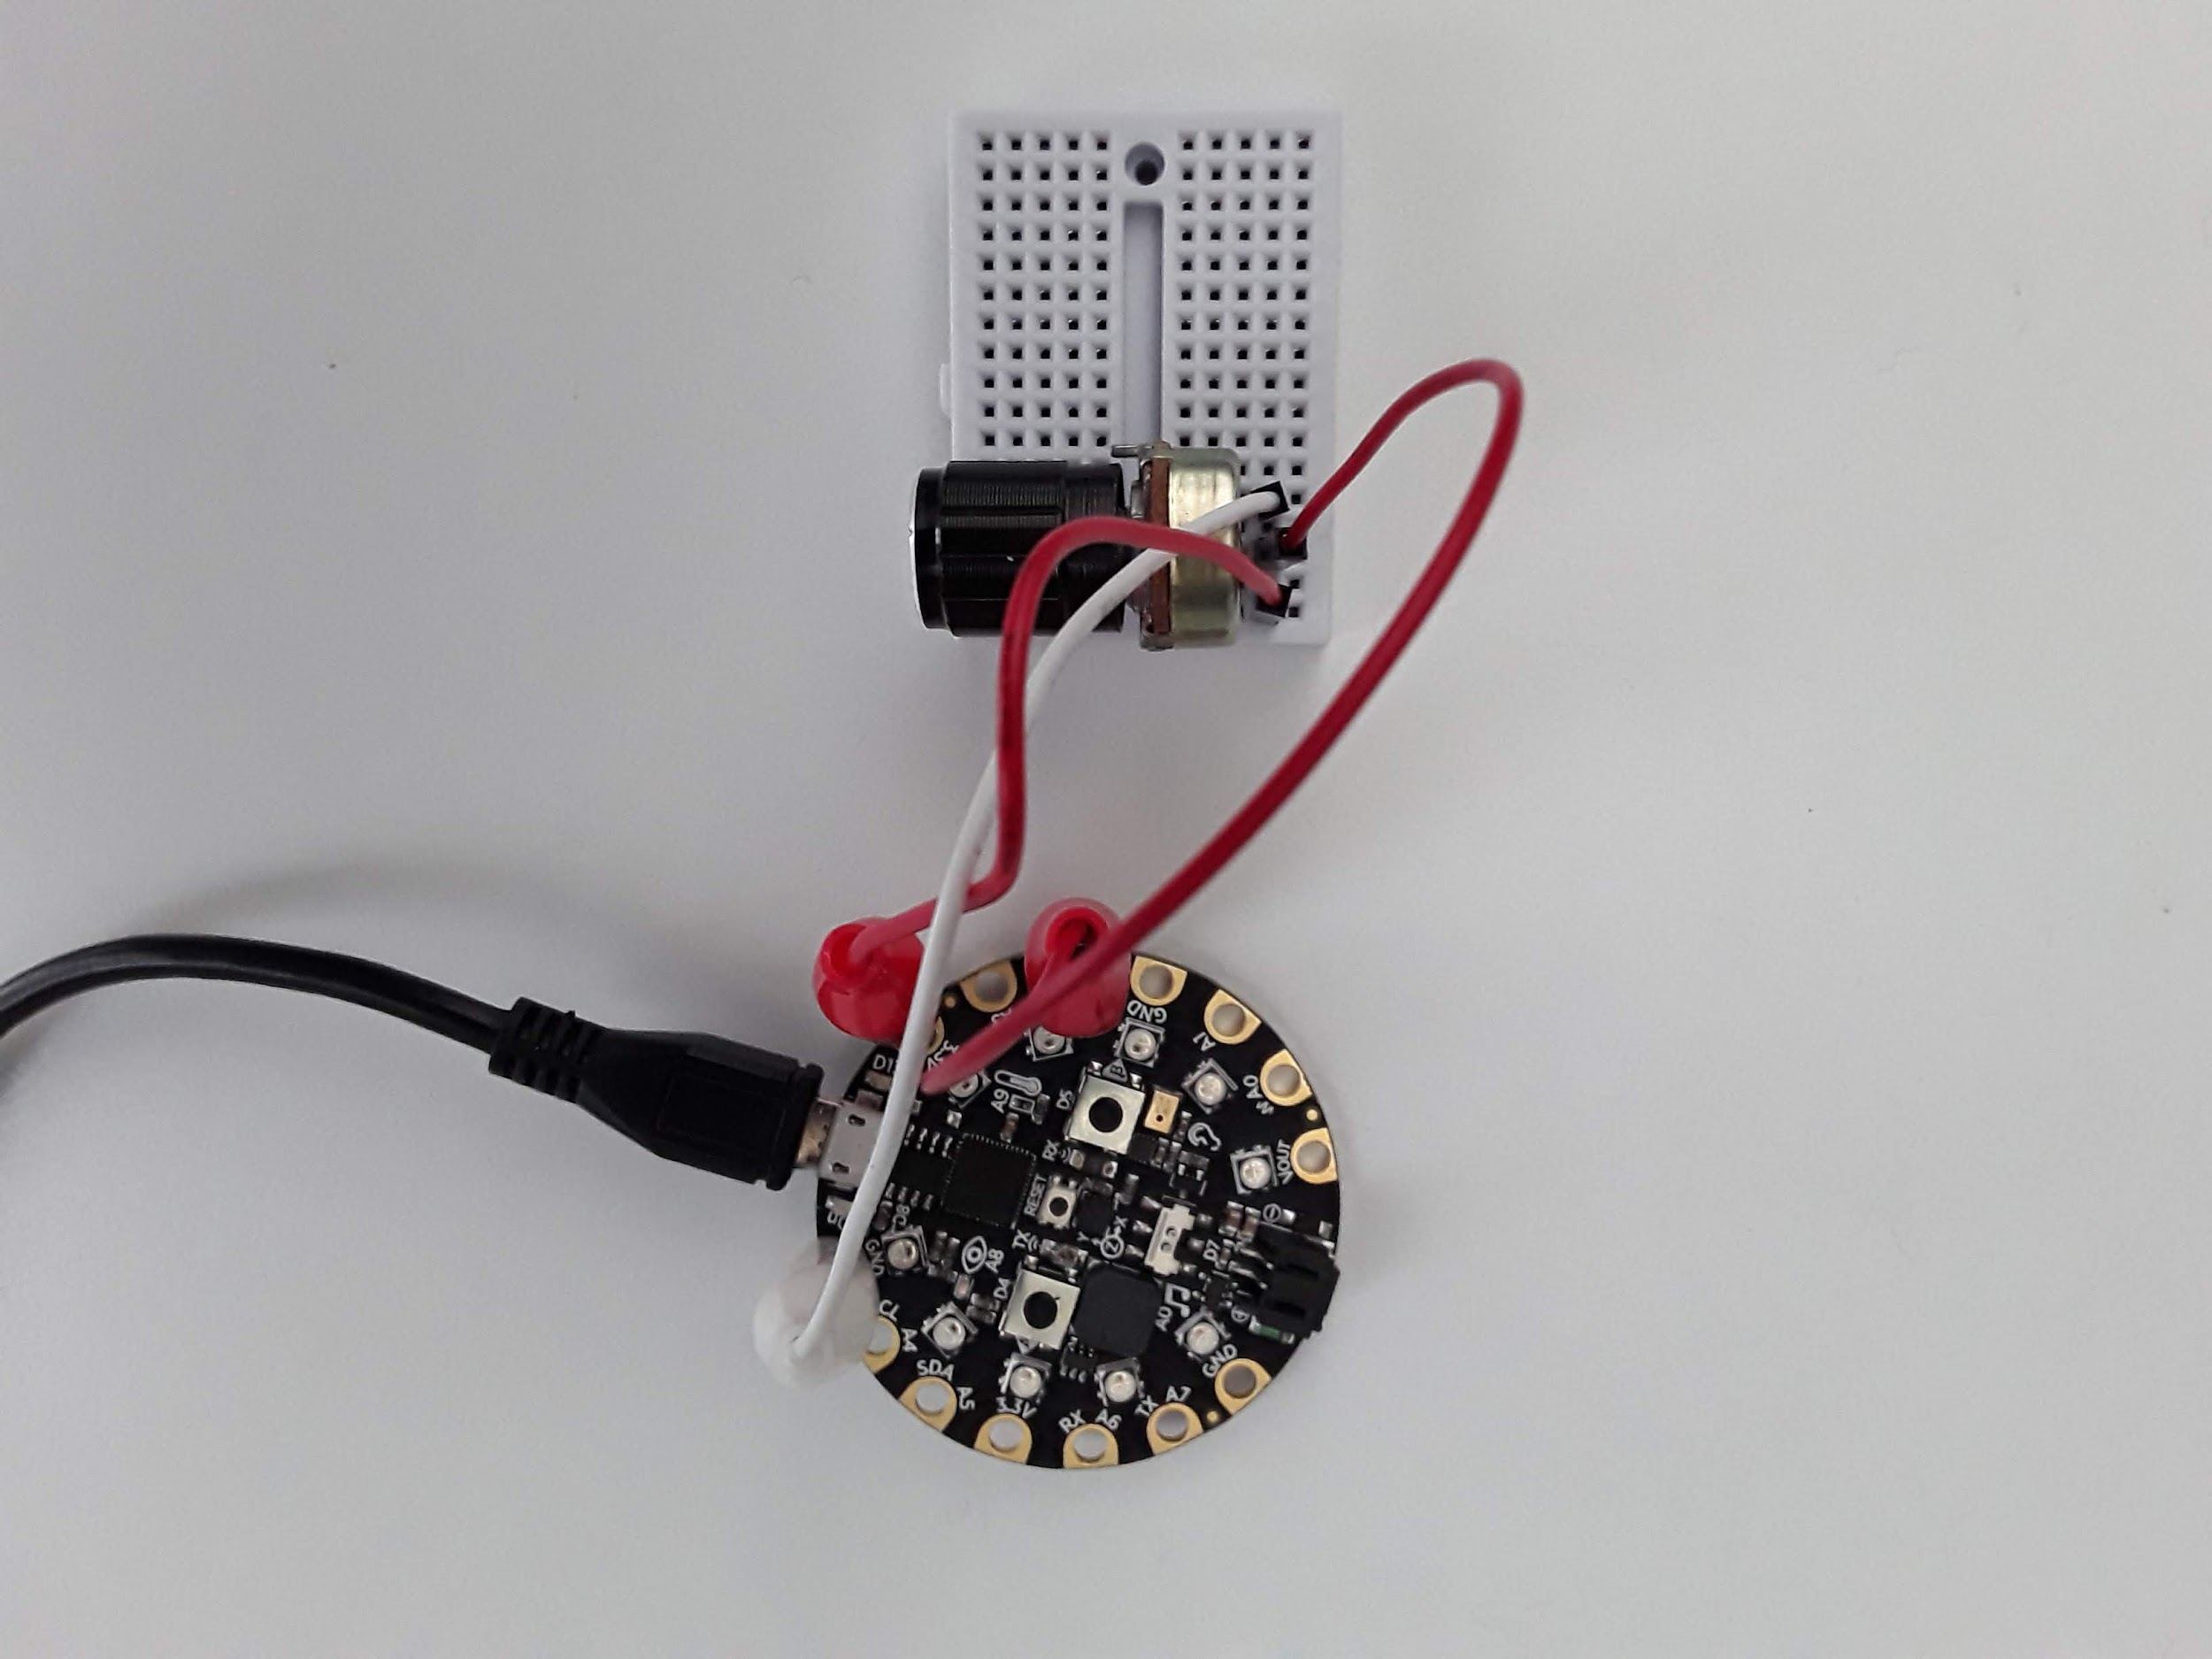
\includegraphics[width=\textwidth]{Figures/potentiometer1.jpeg}
  \end{center}
\end{figure}

\subsection{Assignment}

Upload a PDF with all of the photos and text below included. My
recommendation is for you to create a Word document and insert all the
photos and text into the document. Then export the Word document to a
PDF. For videos I suggest uploading the videos to Google Drive, turn
on link sharing and include a link in your PDF.
\begin{enumerate}[itemsep=-5pt]
\item Use method 1, 2 or 3 and save time and button presses to a text file
\item Include a video explaining which method you are using to record button presses and show yourself pressing the CPX button a few times and recording data. Make sure to wave and introduce yourself - 30\%
\item Copy and Paste your CPX code used to log data - 20\%
\item Copy and paste your Python desktop code used to plot your data - 20\%
\item Include a plot of your button presses with time on the x-axis and button presses on the y-axis (no screenshots) - 30\%
\end{enumerate}
